\section{The Poet and the Sacred}

\begin{wrapfigure}{rt}{.3\textwidth}
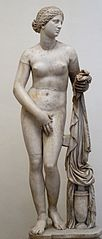
\includegraphics[width=.3\textwidth]{102px-CnidusAphrodite.jpg}
\end{wrapfigure}

The most ancient Traditions are expressed in the form of poetry as, for example, in the Hindu Mahabharata, which includes the Bhagavad Gita, or the poems of \textbf{Homer}. These poems were originally sung, rather than read, by the priests or wandering cantors. As we have pointed out\footnote{\url{https://gornahoor.net/?p=1374}}, poetry reaches a primordial part of consciousness, beyond, and prior to, the reasoning mind.

Following \textbf{Vladimir Solovyov}, art reveals the universal in the particular. The modern mind, which expects uniformity in space and time, has trouble dealing with revelations which occur in a particular place at a particular time. Space and time are qualitative rather than quantitative, so only the intuitive mind can grasp it. The grasping of the whole in poetry is one step removed in grasping the totality of the Absolute.

The recovery of Tradition in the West will necessitate the recovery of the great initiates of Magna Graecia. We start with Pythagoras. \textbf{Virgil} begins with Troy, to describe the founding of Rome, which was the ecumene\footnote{\url{https://en.wikipedia.org/wiki/Ecumene}}, the known world. \textbf{Dante} continues the story with his great synthesis.

We bring three selections, all objectively unrelated to each other, but subjectively expressing the same understanding. \textbf{Virgil}'s \emph{Eclogues} was believed by the Medievals to be a prophecy of the new age to come, which we celebrate at Christmas. If modern minds can no longer grasp it, so much the worse for them. The second selection is from \textbf{Guido De Giorgio}'s \emph{Aforismi e Poesie}. The third is taken from \emph{Iota Unum} by \textbf{Romano Amerio}, again showing the inner connection between the ancient civilization of the pagans and that of the Middle Ages.

\paragraph{Eclogues}
\begin{verse}
The final age of Cumae\\
And the virgin damsel has now arrived,\\
And the reign of Saturn and Rhea returns.\\
The centuries of the Golden Age return.\\
Again the heavens send us long years\\
And new people born of them.\\
Thou, chaste Moon, full of joy,\\
Favour, since thy Apollo now reigns,\\
The Child who was born this day.\\
He alone will cast iron out of the world\\
And populate both Poles with\\
A most precious lineage of gold.
\end{verse}

\paragraph{The Poets}


The Poets, after the Saints, seem to me to be closer to God because, in a certain sense, they spiritualize matter, they lighten it, rendering it ethereal, impalpable.

Poetry is the crown of life, Holiness is the crown of heaven. The poet is more than man, but the Saint is more than the poet. But at one time the Poet was also a Saint when he was not singing of the world, but of God, when he contemplated the world according to God, when he thought while singing, and sang while thinking.

Plato says that the Poet is a ``winged and light being'' who wanders like a bee in the groves of the Muses, gathering the nectar and transforming it into honey ... and he sings like one possessed, aroused by God, who, as Dante would say, dictates to their inner being, and this God is Love ... It is life renewed by the Spirit, no longer a place of wandering, but of conquests and redemption. Consider Virgil: how many poets did he not remove from error, on the road of the Truth of God, he who went, Dante says, like a man, who has a lamp in hand and will bring light for those who lead him but not himself:

\begin{quotex}
\begin{verse}
You did what he does who travels by night,\\
and carries a lamp behind him, that does not help him,\\
but makes those who follow him, wise
\end{verse}

\flright{\textit{Purgatory} XXII: 67-69}
\end{quotex}


Here is the awesome drama of the poets who sometimes save but do not save themselves, who illumine others but not themselves, who return to prison after unchaining the others ... Who will ever sing the drama of Virgil who at the apparition of Beatrice, leaves Dante and takes up again the way of Limbo? ... He, Lucifer, returns to the shadows and lives there ``without hope and in desire... ''

And Brunetto Latini? The Masters of eternity who are excluded from joyful eternity ... These are among the most terrible secrets of the Justice of God which could lead the most steadfast to doubt ... it is necessary to believe awfully in God in order not to waver, not to doubt, to accept what is repugnant to our human reason, to exalt the Lord in everything, in the good, in the evil that He permits, in the implacability of His justice and the apparent injustice of his Mercy. He who is hidden to us to lead us into temptation, to test our resoluteness, to strengthen our faith, to inflame our love, and give wings to our hope.

\paragraph{The Breadth of the Christian ideal}


When we remember the breadth of the Christian idea, it becomes clear that the Renaissance was a revival of that breadth, leading the Christian religion to realize the kinship uniting it to past civilizations within which, buried in sleep, there lay the values of natural religion, ideal beauty, the civic life and such treasures as the \emph{Phaedo}, the \emph{Metaphysics}, the Venus of Knidos, the Parthenon, Homer, and Virgil.

Religion has an expressive capacity much greater than can appear in any one period: it comes out in successive developments which are not always complete in themselves but which, taken as a whole, tend towards a progressive perfection. This growth is hinted at in the Gospel parables of the seed, and in St. Paul's references to the Church in an organism that grows up to the full measure of perfection.

Nor should it be thought that this assimilation of classical culture began with the Renaissance and the flight of Greek refugees from Islam, since it was in fact begun long before, in the midst of the Dark Ages but the monastic preservation of Greek and Latin authors. They were preserved not because the monks found incentives or nourishment for their devotion in Virgil and Horace, but because, quite distinct from the all-pervasive ascetical inspiration of that period, the monks appreciated another ideal which although not ascetic, was nonetheless religious if Christianity does acknowledge the value of earthly things while directing themselves towards heaven.

Furthermore, the blending of ancient civilization with the Christian idea had already happened before the Renaissance in the primordial form of intellectual development, namely poetry; especially in Dante's Divine Comedy, in which the myths, thought and aspirations of the classical world are powerfully combined with the Christian outlook in a daring synthesis. The limbo of the pagans, in which the light of natural wisdom, while not bringing salvation, nonetheless preserves man from the fullness of damnation, is an outstanding intuition of the medieval genius, which was well aware of the spiritual spaciousness of the Christian ideal that both includes, and extends beyond, the ascetic world of the cloister.


\flrightit{Posted on 2012-12-20 by Cologero}

\begin{center}* * *\end{center}

\begin{footnotesize}
\begin{sffamily}
\texttt{william zeitler on 2012-12-22 at 07:44 said:}

Another noteworthy sacred poem in the West would be The Book of Job in the Hebrew Bible (6th-4th century BCE?). Except for a brief prose prologue and epilogue, the entire book is in poetic form.

\hfill

\texttt{Cologero on 2012-12-22 at 09:07 said:}

Thanks for bringing that up Mr. Zeitler. The Book of Job had a large role in the formation of the Medieval mind because of the commentary on it by Gregory the Great, ``Magna Moralia''.


\hfill

\end{sffamily}
\end{footnotesize}

